\section*{{Problem 2: Hashing: Worst-case-Analyse}} 

Sei $A$ eine Hashtabelle der Größe $N$ , und $n \in N$ beliebig. Zeigen Sie: Für jede Schlüsselmenge $K$ mit $|K| \geq (n - 1)N + 1$ und jede Hashfunktion $h : K \rightarrow \{0,\dots, N - 1\}$ existiert eine Menge $S \subseteq K mit |S| = n$, so dass alle Elemente von $S$ auf denselben Eintrag in $A$ abgebildet werden. Was bedeutet das für die worst-case Laufzeit von Hashing mit Verkettung? Wie verträgt sich das mit der Analyse aus der Vorlesung?\\

\noindent
\textbf{Gegeben:}
\begin{itemize}
	\item Hashtabelle $A$ mit Größe $N$ und $n \in \mathbb{N}$ beliebig
	\item Schlüsselmenge $K$ mit $|K| \geq (n-1)N+1$
	\item Hashfunktion $h:K \rightarrow \{0, \dots, N-1\}$
\end{itemize}

\noindent
\textbf{Gesucht:}
\begin{itemize}
	\item Menge $S \subseteq K$ mit $|S| = n$ $|$ so dass alle Elemnte von $S$ auf denselben Eintrag in $A$ abgebildet werden.
	\item Was bedeutet das für die worst-case Laufzeit von Hashing mit Verkettung?
	\item Wie verträgt sich das mti der Analyse aus der Vorlesung?
\end{itemize}

\noindent
\textbf{Lösung:}
\begin{itemize}
	\item $|K| \leq (n-1)*N+1)$ Schlüssel
	\item Hashtabelle $A$ der Größe $N$
\end{itemize}
$\Rightarrow$ Schubfachprinzip:\\
Kugeln: Schlüssel $((n-1)N+1)$\\
Fächer: Hashtabelle $(N)$\\
Zuordnung: Schlüssel durch die Hashfunktion in die jeweilige Hashtabelle einordnen\\

$\rightarrow$ Wir wollen die Teilmenge $S \subseteq K$ von Größe $n$, die alle denselben Hashwert haben $\rightarrow$ also im selben Fach landen.\\
$\rightarrow$ wir wollen höchsten $n$ Schlüssel im selben Fach haben\\
$\Rightarrow$ wir wollen also maximal $n-1$ Schlüssel in jedem Fach, außer einem mit $n$ Schlüsseln haben:\\

\begin{center}
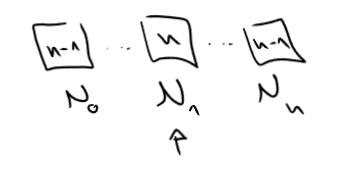
\includegraphics[scale=0.5]{Schubfach_skizze}
\end{center}

$\rightarrow$ d.h. wenn wir wissen möchten wie viel Schlüssel wir pro Slot(Fach) haben können wir das so ausdrücken: $n-1$\\

$\Rightarrow$ Wenn wir wissen möchten wie viel Schlüssel wir also maximal haben: $(n-1) * N$ $|$ $*N \text{ anzahl der Fächer}$\\
$\rightarrow$ damit kriegen wir für jedes Fach maximal $n-1$ Schlüssel!\\
Nach der Aufgabenstellung haben wir aber mehr Gegeben!:\\

$|K| \geq (n-1)*N+1$\\

\noindent
$\Rightarrow$ Demnach haben wir genau ein Schlüssel mehr als wir brauchen und somit auch ein Fach was mehr als $n-1$ Schlüssel hat und genau $n$ Schlüssel. Dies bildet die gesuchte Menge $S \subseteq K$, mit $|S|=n$ und $\forall x \in S:h(x)=i$ für irgendein $i \in \{0, \dots, N-1\}$\\
\begin{flushright}
$\Box$
\end{flushright}

\noindent
\textbf{Beispiel:}
\begin{itemize}
	\item Fächer $N$: 5
	\item Schlüssel $n$ = 8
	\item $\Rightarrow$ $(n-1)*N+1=(8-1)*5+1=36$
	\item $36$ auf $5$ Fächer sind:
	\begin{itemize}
		\item $4$ Fächer mit $7$ Schlüsseln \&
		\item $1$ Fach mit $8$ Schlüsseln\\
	\end{itemize}
\end{itemize}

\noindent
\textbf{Was bedeutet das für die worst-case Laufzeit von Hashing mit Verkettung?}

\begin{itemize}
	\item Bei Hashing mit Verkettung speichern wir alle Schlüssel, die denselben Hashwert haben, in einer Liste in der jeweiligen Stelle der Hashtabelle
	\item d.h. im worst-case kann es passieren, dass alle Schlüssel auf denselben Slot gespeichert werden (z.B. bei schlechter Hashfunktion)
	\item Im Schlimmsten Fall muss man also eine Liste mit $n$ Elementen durchsuchen
\end{itemize}
\textbf{Worst-Case-Laufzeit für Hashing mit Verkettung ist also:}\\
$\Rightarrow$ $O(n)$\\

\noindent
\textbf{Wie verträgt sich das mit der Analyse aus der Vorlesung?}
\begin{itemize}
	\item In der Vorlesung wird für Hashing mit Verkettung eine Laufzeit von $O(1+ \frac{n}{m})$ angegeben
	\item $\frac{n}{m}$ ist hierbei der Ladefaktor $n$: Schlüssel, $m$: die Größe der Hashtabelle(Slots)
	\item Im besten Falle sollte der Ladefaktor zwischen 1 \& 3 sein. Hierbei handelt es sich also um die Praktische Anwendung von Hashing mit Verkettung oder auch Average-Case-Laufzeit
	\item Bei gute Wahl vom Ladefaktor kann also die Laufzeit $O(1)$ werden, wenn der Ladefaktor zu $\approx 1$ wird
	\item Im Vergleich haben wir also den Worst-Case von $O(n)$ und den Average-Case von $O(1)$
\end{itemize}